\documentclass[12pt,a4paper,titlepage]{article}

\usepackage{preamble}

\title{MSTAT : Travaux pratiques}
\author{Yassine Jamoud, Samy Haffoudhi}
\date{\today}
\usepackage{mathtools}

\renewcommand{\theenumi}{\alph{enumi}}

\begin{document}

\maketitle

\section*{Introduction}

Dans cet exercice nous considérons un moteur à courant continu commandé
par la tenson d'induit $u(t)$. La position angulaire du rotor $\theta(t)$ est mesurée par
un codeur incrémental à $L$ = 521 lignes par tour, fournissant une mesure $y(t)$ de $\theta(t)$.
$\Omega(t)$ est la vitesse de rotation. On cherche alors à estimer en ligne $\theta(t)$
et $\Omega(t)$ connaissant $u(t)$ et $(y(t)$.

\setcounter{section}{5}

\section{Filtrage de Kalman}

\subsection{Synthèse de l'entrée du système}

$u(t)$ est un créneau centré de période $\Delta$ = 100 ms, d'amplitude crête à crête
$A$ = 0,1 V. Ce signal est échantillonné à la période $T_e$ = 1 ms. Programmons une
fonction Matlab permettant de synthétiser cette entrée échantillonnée pour une durée D.

\lstinputlisting[language=Matlab]{../entree.m}

\begin{figure}[H]
    \caption{Entrée du système}
    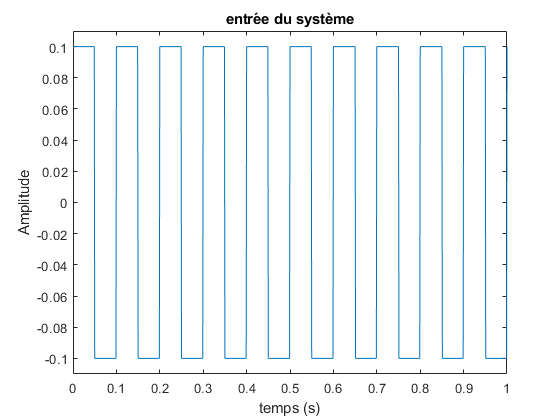
\includegraphics[width=0.5\textwidth]{entree}
    \centering
\end{figure}

\subsection{Modélisation et simulation du système}

\begin{enumerate}

    \item{Programmons le simulateur :
            \lstinputlisting[language=Matlab]{../simule.m}
        }

    \item{Testons alors ce simulateur avec $G$ = 50 rad.$s^{-1}$.$N^{-1}$ et $T$ = 20 ms.
            On obtient les tracés suivants :

            \begin{figure}[H]
                \caption{Mesure de la position angulaire}
                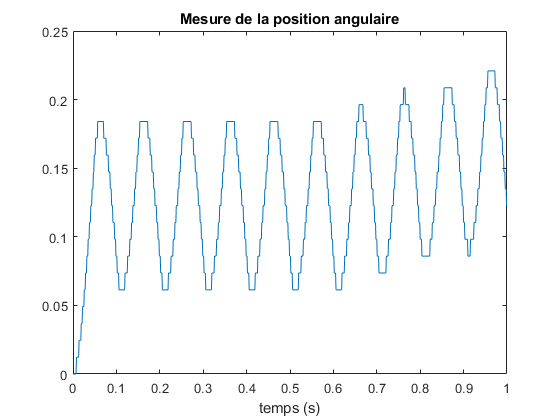
\includegraphics[width=0.5\textwidth]{simule1}
                \centering
            \end{figure}

            On dérivant $y$, on obtient :

            \begin{figure}[H]
                \caption{Vitesse de rotation}
                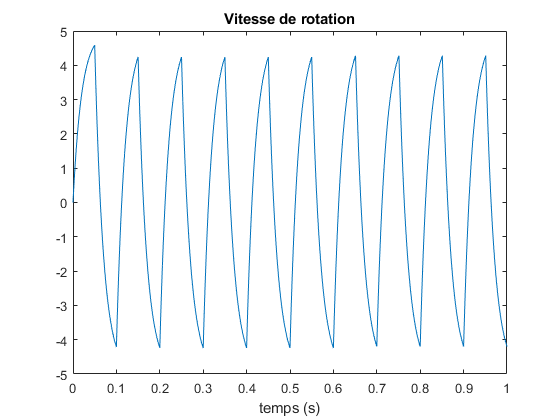
\includegraphics[width=0.5\textwidth]{simule2}
                \centering
            \end{figure}
        }

\end{enumerate}

\subsection{Estimation par filtrage de Kalman}

\begin{enumerate}

    \item{Écrivons la représentation d'état stochastique du modèle du systèe d'entré 
            $u_n$ et de sortie $y_n$ :

            \begin{cases}
                y_n &= H_n X_n + h_n + w_n \\
                X_{n+1} &= F_n X_n + f_n + v_n
            \end{cases}

            Avec,

            \begin{itemize}
                \item{$h_n = 0$}
                \item{$H_n = 
                        \begin{bmatrix}
                            1 & 0\\
                        \end{bmatrix}
                    $}
                \item{$C_{w_n,w_n} = r$}
                \item{$F_n = \tilde{A}$}
                \item{$f_n = \tilde{B}$}
                \item{$C_{v_n,v_n} = q$}
            \end{itemize}
        }

    \item{r correspond à la variance du bruit de mesure blanc du codeur incrémental. On
            propose alors une valeur correspond à la variance d'une variable suivant la
            loi uniforme sur $[0, 2 \pi / L]$ étant donné la précision du codeur incrémental
            à L lignes par tour :

            $$r = \frac{(2\pi/L)^2}{12}$$
        }

    \item{Le moteur est non alimenté et à l'arrêt avant le premier instant d'échantillonnage
            mais nous disposons d'aucune information sur la position angulaire initiale.

            On propose alors étant donné ces connaissances :

            \begin{cases}
                \hat{X}_{1/O} &= 0 \\
                P_{1/0} &= \frac{2\pi}{12}
            \end{cases}
        }

    \item{Programmons le filtre de Kalman optimal :

    \lstinputlisting[language=Matlab]{../kal.m}

    Et le filtre de Kalman statique :

    \lstinputlisting[language=Matlab]{../kal_statique.m}
        }

    \item{Pour le cas d'un système parfaitement modélisé :

            \begin{figure}[H]
                \caption{Estimations (système parfaitement modélisé)}
                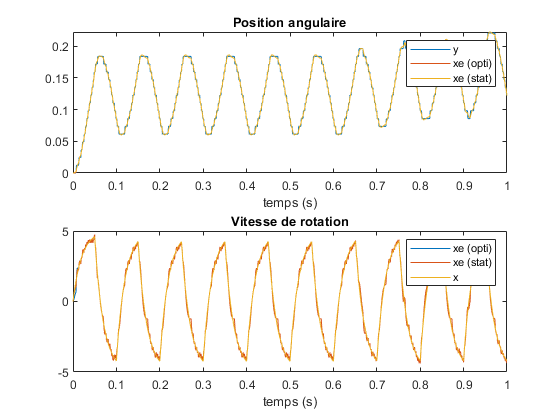
\includegraphics[width=0.5\textwidth]{kal1}
                \centering
            \end{figure}

            Pour une modélisation imprécise :

            \begin{figure}[H]
                \caption{Estimations (modélisation imprécise)}
                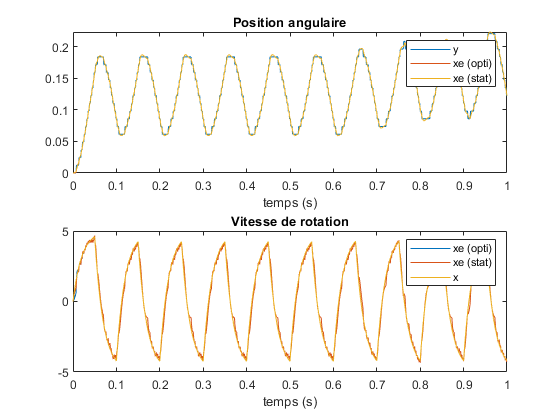
\includegraphics[width=0.5\textwidth]{kal2}
                \centering
            \end{figure}
        }

\end{enumerate}

\begin{enumerate}

\end{enumerate}

\end{document}
